%%%%%%%%%%%%%%%%%%%%%%%%%%%%%%%%%%%%%%%%%
% University/School Laboratory Report
% LaTeX Template
% Version 3.1 (25/3/14)
%
% This template has been downloaded from:
% http://www.LaTeXTemplates.com
%
% Original author:
% Linux and Unix Users Group at Virginia Tech Wiki 
% (https://vtluug.org/wiki/Example_LaTeX_chem_lab_report)
%
% License:
% CC BY-NC-SA 3.0 (http://creativecommons.org/licenses/by-nc-sa/3.0/)
%
%%%%%%%%%%%%%%%%%%%%%%%%%%%%%%%%%%%%%%%%%

%----------------------------------------------------------------------------------------
%	PACKAGES AND DOCUMENT CONFIGURATIONS
%----------------------------------------------------------------------------------------

\documentclass[UTF8]{ctexart}

\usepackage{siunitx} % Provides the \SI{}{} and \si{} command for typesetting SI units
\usepackage{graphicx} % Required for the inclusion of images
\usepackage{graphics}%图片设置
\usepackage{subfigure} 

\usepackage{natbib} % Required to change bibliography style to APA
\usepackage{amsmath} % Required for some math elements 
\usepackage{amssymb} % 使用因为所以符号
\usepackage{fancyhdr} % 使用页眉

\usepackage{algorithm}
\usepackage{algorithmic}

%\usepackage{url} % 引用URL
% \usepackage{cite}
% \newcommand{\upcite}[1]{\textsuperscript{\textsuperscript{\cite{#1}}}} %参考文献上标

\pagestyle{fancy}
\fancyhf{} 
\cfoot{\thepage} 

\setlength\parindent{0pt} % Removes all indentation from paragraphs

\renewcommand{\labelenumi}{\alph{enumi}.} 

%----------------------------------------------------------------------------------------
%	DOCUMENT INFORMATION
%----------------------------------------------------------------------------------------
\title{算法分析与设计-作业三}

\author{王宸昊 2019214541}

\date{\today}

\begin{document}

\maketitle

%----------------------------------------------------------------------------------------
%	SECTION 1
%----------------------------------------------------------------------------------------

\section{CLRS, Page, 112 8.3-4}

证明: \\
借鉴基数排序的思想,将取值从0到$n^3-1$的n个整数,用n进制来表示,即每一位都是0到n-1的正整数,则最多用$log_n(n^3)=3$位可以表示$n^3$个整数。\\
根据P.111的引理8.3可知,排序的时间复杂度为$\varTheta(3(n+n)) = \varTheta(n)$,满足$O(n)$。

%----------------------------------------------------------------------------------------
%	SECTION 2
%----------------------------------------------------------------------------------------

\section{CLRS, Page, 114 8.4-4}

证明:\\
借鉴桶排序的思想,关键问题将点的分布均匀的映射到不同的桶中。因为所有的点服从均匀分布,所以将半径为1的圆,根据面积等分为n份,即等分为n个面积为1/n的圆环,则第i个圆盘的半径满足:

\begin{align*}
    \pi({r_i}^2-{r_{i-1}}^2) &= \frac{\pi}{n} \\
    {r_i}^2-{r_{i-1}}^2 &= \frac{1}{n}\\
    \vdots\\
    {r_2}^2-{r_{1}}^2 &= \frac{1}{n}
\end{align*}

因此,由上式的递推公式可得,第i个圆环的半径为$r_i=\sqrt{\frac{i}{n}}$。\\
则对应桶的半径区间为$[0,\sqrt{\frac{1}{n}}), [\sqrt{\frac{i}{n}}, \sqrt{\frac{2}{n}}), \ddots, [\sqrt{\frac{n-1}{n}}, 1) $。

由上所知共有n个桶,根据下面公式,即可由每个点的d得到应放在第k个桶内:

\begin{equation*}
    k=\left\{
    \begin{array}{rcl}
    \left\lfloor d * n\right\rfloor + 1 & & {d < 1}\\
    n & & {d = 1}
    \end{array} \right.
\end{equation*}
  
%----------------------------------------------------------------------------------------
%	SECTION 3
%----------------------------------------------------------------------------------------

\section{对比不同排序算法的排序效果}

\subsection{算法简介}

\textbf{插入排序:}\\
插入排序的算法思想是在排序数组的前面维护一个有序的子集,当遍历的元素存在逆序时,将前面的元素依次后移,找到当前元素合适的插入位置插入。对于一个无序数组A[1...n],i表当前待排序元素,A[1...i-1]的元素都已经是排序好的元素,则只需要找到A[i]的小的元素,在其后面插入即可。由于遍历整个数组有n个元素,而依次移动前面的元素复杂度为O(n),整体的复杂度为$O(n^2)。$\\

\textbf{快速排序:}\\
快排利用里分治的思想,对待排序数组A[p...r],划分为两个数组A[p...q-1], A[q+1...r],其中A[p...q-1]的每一个元素都小于A[q], A[q+1...r]的每一个元素都大于A[q],随后再依次递归排序两个子数组。按照平均的算法度进行分析,算法复杂度的平均期望为$O(nlgn)$。\\
需要注意的是,对于划分位置的选择很大程度上影响了算法的平均执行时间,在本实验的解决方案是随机选择一个位置,然后与最后一个位置的元素进行交换,保证划分区间尽量均匀。\\

\textbf{归并排序:}\\
归并排序也利用了分治的思想,将待排序数组A[i, j]从mid处中间划分,递归排序子数组A[i, mid],A[mid, j],最后再归并两个有序的子数组。从时间复杂度上看,归并排序的时间复杂度为$O(nlgn)$,此外,还需要长度为n的数组作为辅助存储,所以空间复杂度O(n)。\\

\textbf{希尔排序:}\\
希尔排序在底层使用插入排序,具体实现是采用不同的增量对数据进行分组,不同组的元素之间进行插入排序,然后缩小增量,再次进行插入排序,最后当增量等于1的时候,再进行插入排序时,整个数组也就是有序数组了,整体上分析,希尔排序的复杂度在$O(n)-O(n^2)$之间。\\
在这里,增量的选取的为3k+1。\\

\textbf{基数排序:}\\
基数排序的算法思想是对n个的数的低位到高位依次进行排序,这样排列出来的数组就是有序的了。假设有n个数字,每一位取值0-9,最多有d位,于是算法的复杂度为$O(d(10+n))$。需要注意的是,可以采用不同k进制数来表示不同的数,这样使用每一轮查看的元素的个数变为n+k,在本次实验中,我们去k=10进制表示。

\subsection{算法实现}

算法的具体实现在src目录下的sort.py当中,使用的语言为python,在程序中分别封装了5中算法的具体实现,在main函数中生成不同规模的随机数据,在这里随机算法选用Python的random()模块,可以产生任意大小的随机数。需要注意的是,为了消除待排序数组的分布对排序结果的影响,对于某一数据规模下的实验,我们对不同算法采用相同的测试集,然后将结果输出到data目录下的data.txt当中。

\subsection{实验环境}
编译环境为Python3.7,操作系统的版本为Windows 10。\\
CPU为AMD Ryzen 7 1700(3.0 GHz),RAM 16G。\\
第三方模块:
\begin{itemize}
\item time(): 对算法执行过程进行高精度的计时,最高精度可达微秒级别
\item random(): 产生任意大小的随机数
\item sys():查看内存使用情况
\end{itemize}

\subsection{实验结果}
在不同的数据规模下,测试的结果如图\ref{compare}所示:

\begin{figure}[H]
    \centering
    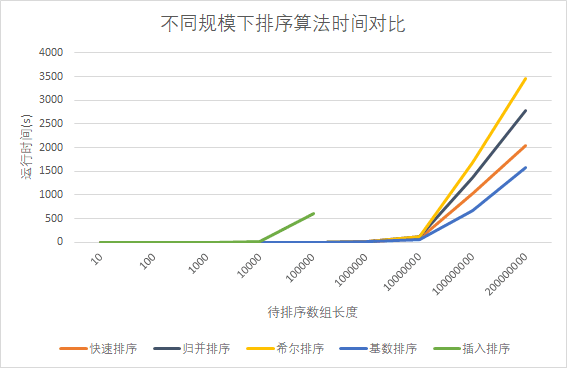
\includegraphics[width=1\textwidth]{img/compare.png}
    \caption{不同规模下排序算法时间对比}
    \label{compare}
\end{figure}

首先关注插入排序的运行时间,在10000个待排序数时,时间消耗是6.076秒,而在100000个数的时候,运行时间迅速增长到了599.576秒,由此可以看出复杂度$O(n^2)$的算法的增长是非常快的,在1000000的数据规模的时候,已经在有限时间内已经计算不出结果,所以在图中没有后续的数据。\\

从图中的对比中可以看出,在不同的数据规模的下,不同排序算法的表现都比较稳定,执行时间的表现从快到慢分别是:基数排序,快速排序,归并排序,希尔排序。\\
从结果的上进行分析,基数排序从理论的时间复杂度是线性的算法,所以要明显优于基于对比的其他排序算法,这一点也在数据中可以证明。\\
在基于比较的算法中,快排的排序效果比较稳定,在不同的数据规模下明显优于其他算法。\\
归并排序算法在大量数据的情况下,效果并不算突出。希尔排序在大量的数据下,退化也比较严重,在几个基于比较的排序算法中,性能最差。

\subsection{选做部分}

在本机上进行$10^9$规模的实验的时候,会发生MemoryError的错误,如图\ref{error} 所示\\

\begin{figure}[H]
    \centering
    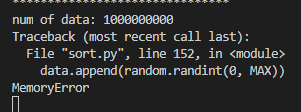
\includegraphics[width=1\textwidth]{img/error.png}
    \caption{MemoryError}
    \label{error}
\end{figure}

究其原因,与Python中无符号整型数的范围有关,在Python中,int类型的数并不会溢出,而是会根据数据的大小动态的申请空间,由于我们每个数的取值范围为$[0,2^{32}-1]$在Python中,每$2^{30}$个数会增加4字节.在最差的情况下,因此从原理上我们的数据需要8个字节来表示,但是按照这种算法,我们需要申请大约8GB的内存就足够分配了,但是为什么在16G的内存下还是溢出了呢?\\

于是我测量了$2^{32}-1$的无符号整数实际在本机上占用的空间大小,如图\ref{size}所示:

\begin{figure}[H]
    \centering
    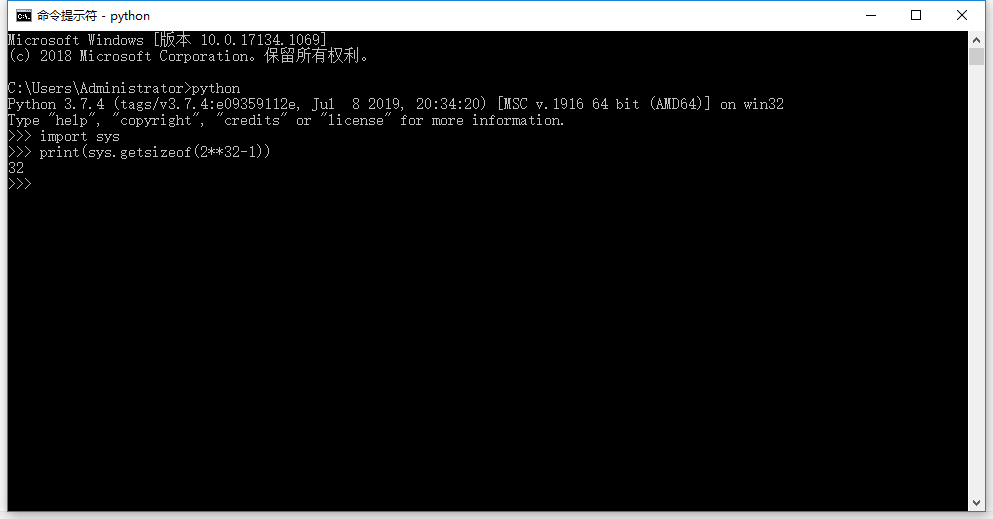
\includegraphics[width=1\textwidth]{img/size.png}
    \caption{无符号整数占用空间}
    \label{size}
\end{figure}

注意这里返回的单位是字节。可以看到返回的结果是32bytes,也就是32字节,为什么会多出这么多位呢,经过一番查证后发现,正是由于在Python中整型不会溢出,根据每台机器上的硬件设备不同,所以需要在每个整型对象头部添加大量的信息。按照这样计算,我们大约需要32GB的内存,16GB的内存也就自然会溢出了。\\

为了解决这个问题,采用最直观的方法,寻找一台内存32GB以上的服务器执行,此次的实验环境为:Ubuntu16.04.10, python3.5.2, CPU:Intel Xeon(R) E5-2620(2.10GHz),内存:128GB。
得到的结果表\ref{table-1}所示。\\
实验环境

\begin{table}[H]
    \caption{$10^9$输入规模下算法性能测试}
    \label{table-1}
    \begin{center}
        \begin{tabular}{cc}
            \hline
            排序算法&   执行时间(s)\\     
            \hline
            快速排序&       13510.133\\               
            归并排序&       17861.703\\              
            希尔排序&       23620.192\\             
            基数排序&      9998.141\\                      
            \hline
        \end{tabular}  
    \end{center}
\end{table}

从上表的数据可以明显的看出,从总体上看,在数据量比较大的时候,排序是一件相当耗时的事情。以快排为例,进行一次排序约3.7个小时。同时可以看出,在基于比较的算法的当中,快速排序的算法的执行时间是最优秀的,基数排序作为一种接近线性的算法,其执行时间明显优于其他基于比较的算法,在10进制的情况下,只需要2.7个小时就可以完成排序。

\end{document}